\documentclass{article}
\usepackage[utf8]{inputenc}

\title{Laboratorio03_INTELIGENCIA_NEGOCIOS}
\author{edwartbalcon}
\date{Septiembre 2021}

\usepackage[utf8]{inputenc}
\usepackage[spanish]{babel}
\usepackage{natbib}
\usepackage{graphicx}

\begin{document}

\title{Caratula}

\begin{titlepage}
\begin{center}
\begin{Large}
\textbf{UNIVERSIDAD PRIVADA DE TACNA} \\
\end{Large}
\vspace*{-0.025in}
\begin{figure}[htb]
\begin{center}

\includegraphics[width=6cm]{./images/logo_UPT}
\end{center}
\end{figure}
\vspace*{-0.025in}
\begin{Large}
\textbf{FACULTAD DE INGENIERIA} \\
\end{Large}
\vspace*{0.05in}
\begin{Large}
\textbf{Escuela Profesional de Ingeniería de Sistema} \\
\end{Large}


\vspace*{0.4in}

\vspace*{0.1in}
\begin{Large}
\textbf{Informe de laboratorio 10: Construyendo una
Arquitectura Serverless} \\
\end{Large}

\vspace*{0.3in}
\begin{Large}
\textbf{Curso: Inteligencia de negocios} \\
\end{Large}

\vspace*{0.3in}
\begin{Large}
\textbf{DOCENTE: Ing. Patrick Cuadros Quiroga} \\
\end{Large}

\vspace*{0.2in}
\vspace*{0.1in}
\begin{large}

\begin{Large}
\textbf{Alumno: Balcon Coahila, Edwart Juan\hfill	(2013046516) } \\
\end{Large}

\vspace*{0.15in}
\begin{Large}
\textbf{Tacna – Perú} \\
\end{Large}

\vspace*{0.05in}
\begin{Large}
\textbf{2021 } \\
\end{Large}

\end{large}
\end{center}

\end{titlepage}


\newpage

\section{ Realizar los siguientes pasos para el laboratorio }

\textbf{1.1.  Visualizamos en CloudFormation que se estén creando los recursos del stack.}

\begin{center}
		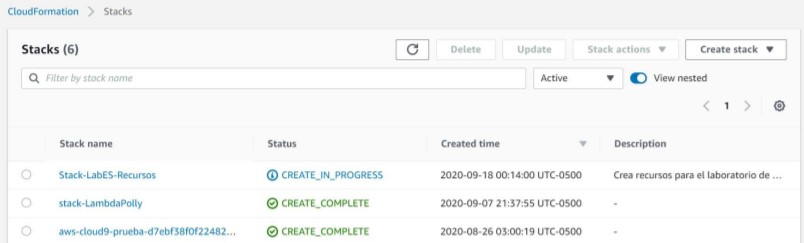
\includegraphics[width=15cm]{./images/1} 
	\end{center}
	
\textbf{1.2. Para hacer una prueba de nuestros token de Twitter, ejecutaremos lo siguiente, pero antes debemos
agregar nuestros token dentro el código.}


    \begin{center}
		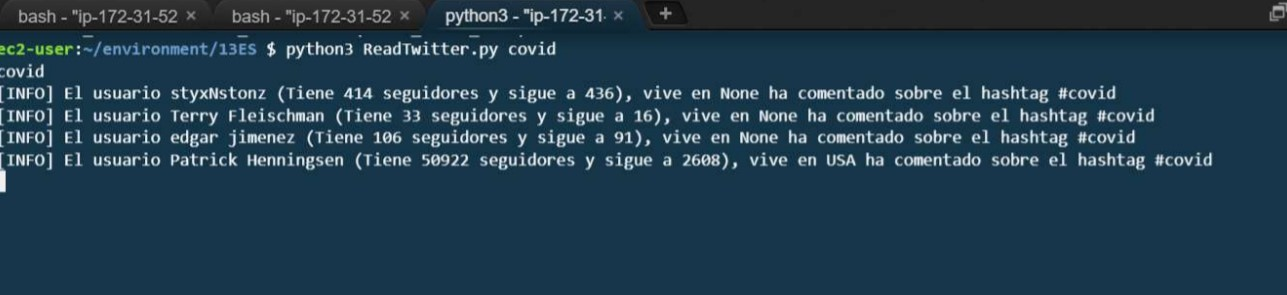
\includegraphics[width=15cm]{./images/2} 
	\end{center}

\textbf{1.3.   Entramos a la carpeta docker.
}

    \begin{center}
		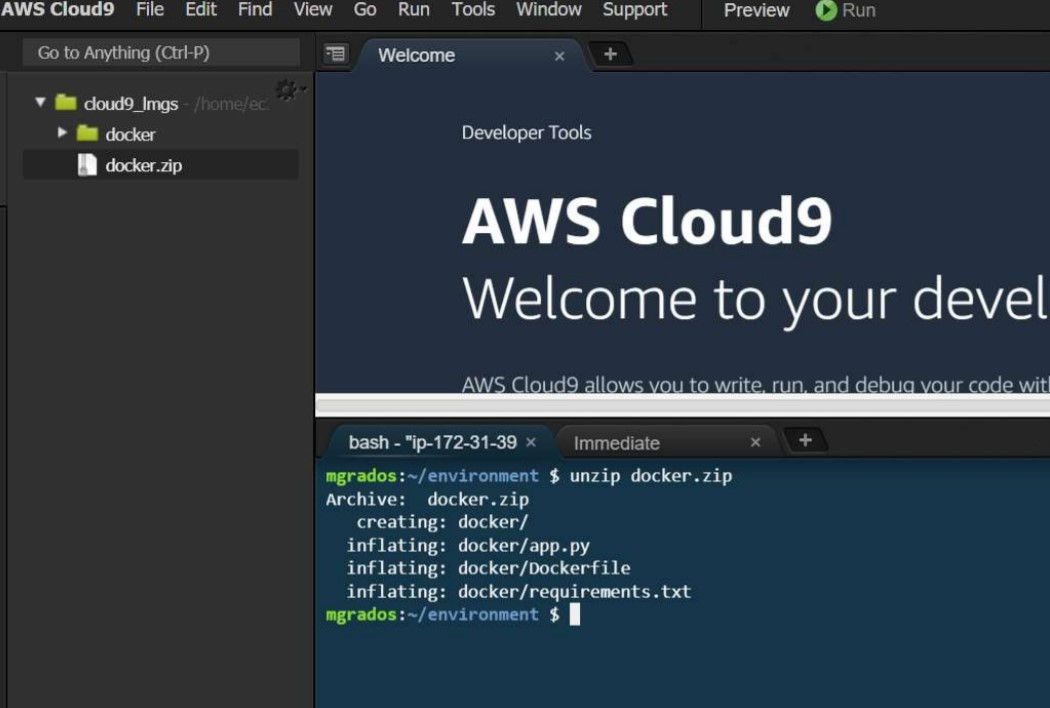
\includegraphics[width=15cm]{./images/3} 
	\end{center}

\newpage
\textbf{1.4.  Entramos al servicio de ECR desde la consola y veremos nuestro repo creado.
Copiamos el URI del repositorio.
}

    \begin{center}
		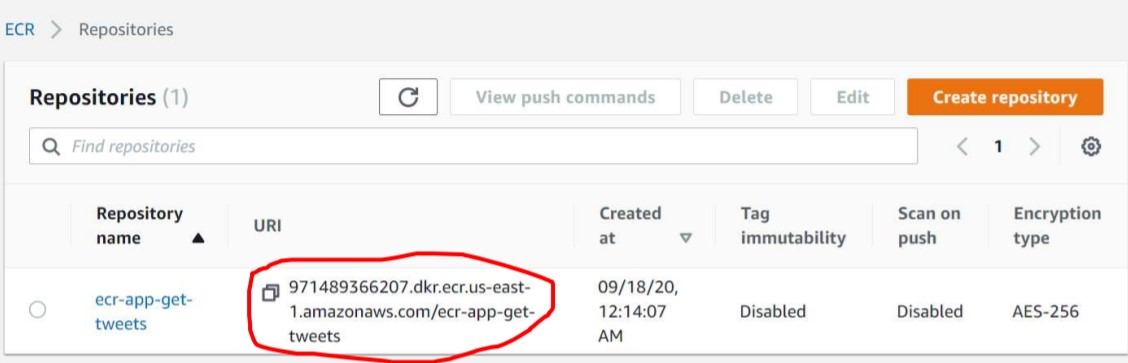
\includegraphics[width=15cm]{./images/4} 
	\end{center}
	
	\newpage
\textbf{1.5.  Construiremos la imagen Docker.
}

    \begin{center}
		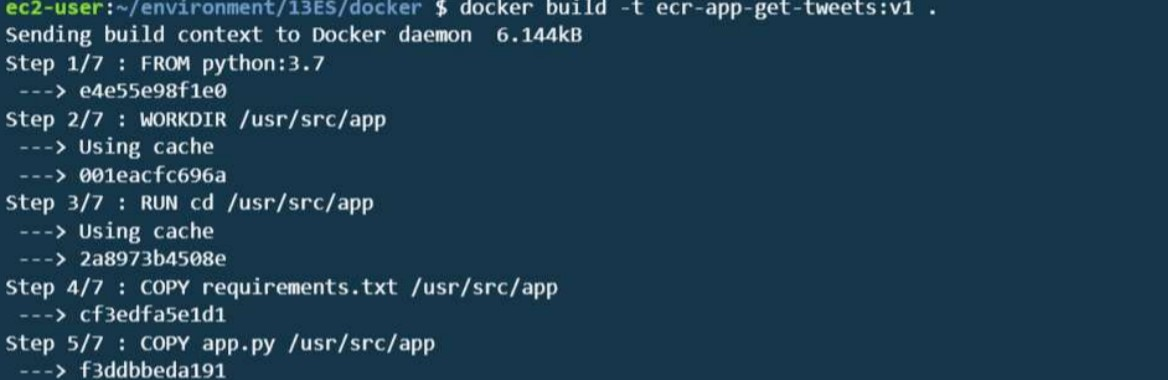
\includegraphics[width=15cm]{./images/5} 
	\end{center}
	
	\newpage
\textbf{1.6.   Subimos la imagen al ECR
}

    \begin{center}
		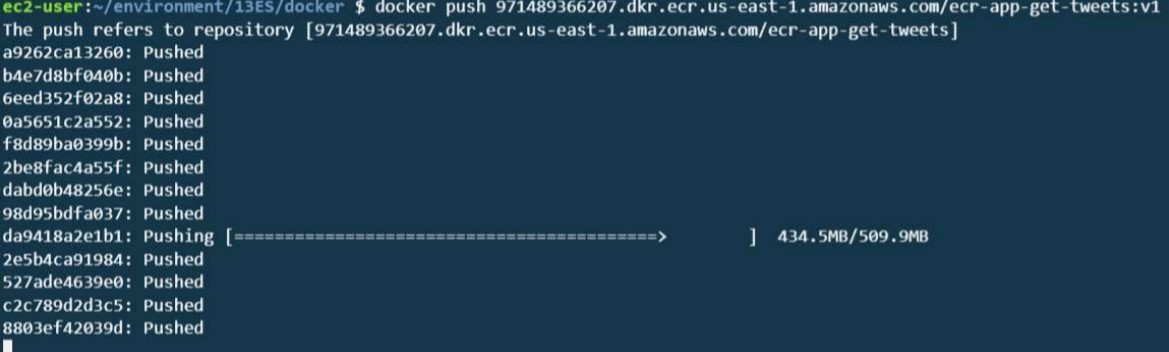
\includegraphics[width=15cm]{./images/6} 
	\end{center}
	
	\newpage
\textbf{1.7. Regresamos el ECR y obtenemos el URI de la imagen subida.
}

    \begin{center}
		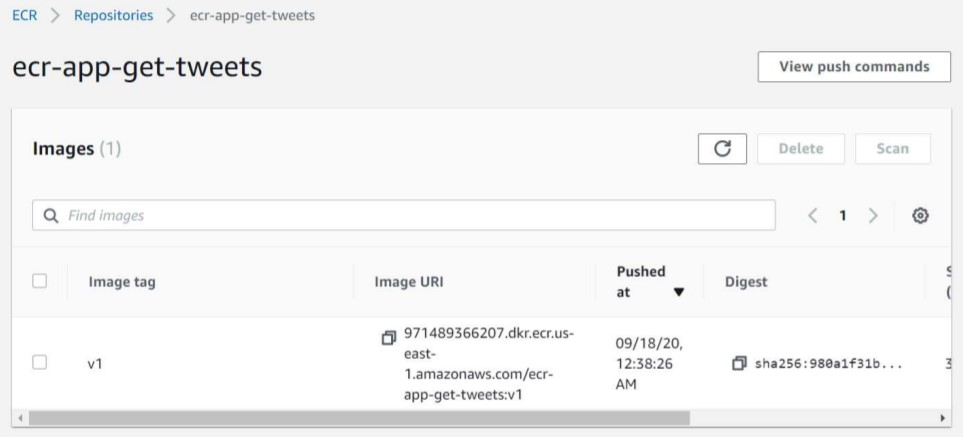
\includegraphics[width=15cm]{./images/7} 
	\end{center}
	
	\newpage
\textbf{1.8.  Seleccionamos el tópico TopicTweetsNegative y obtenemos su ARN y Clic en la función Lambda llamada : DetectSentimentTweets.
}

    \begin{center}
		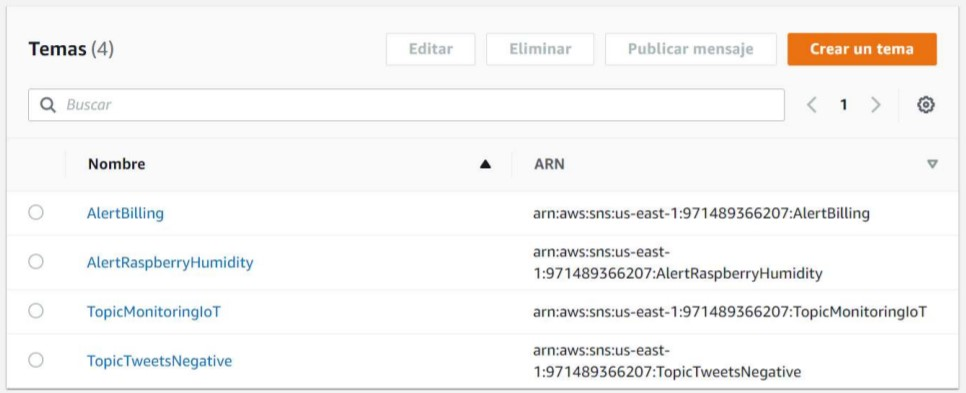
\includegraphics[width=15cm]{./images/8} 
	\end{center}
	
    \begin{center}
		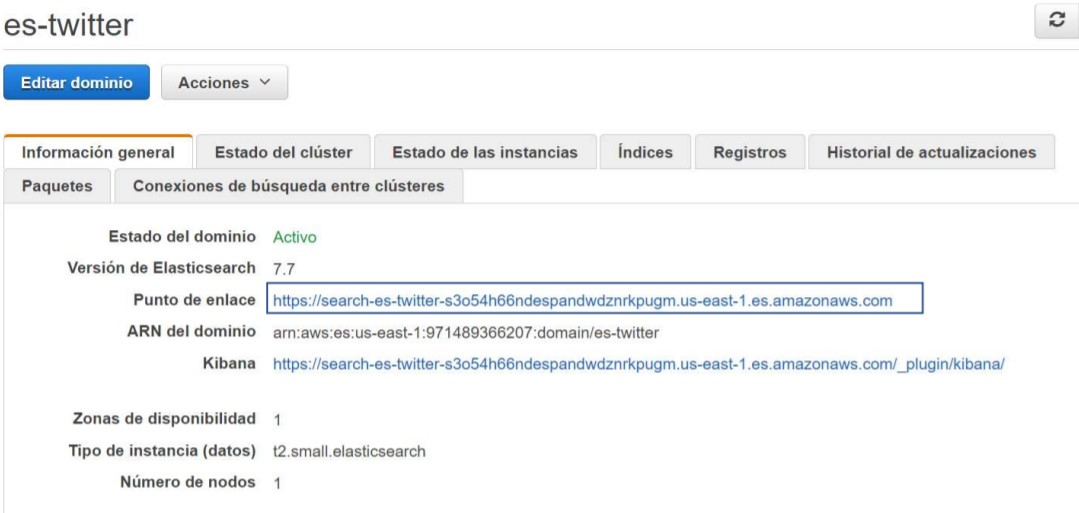
\includegraphics[width=15cm]{./images/9} 
	\end{center}
	
	\newpage
\textbf{1.9.   Creamos un clúster en ECS (no genera costo), clic en Get Started
}

    \begin{center}
		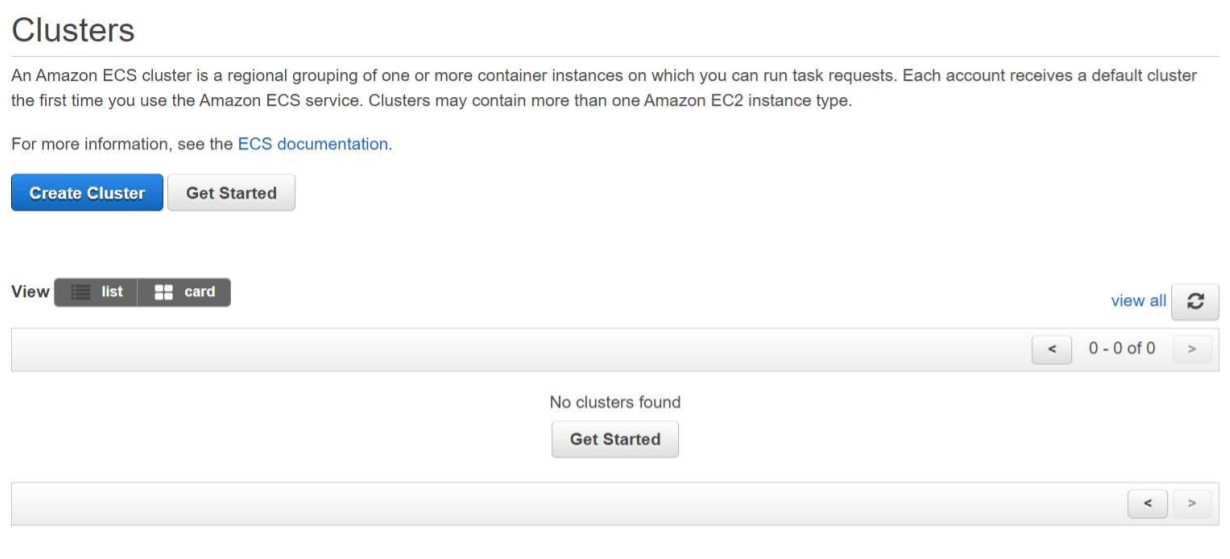
\includegraphics[width=15cm]{./images/10} 
	\end{center}
	
		
	\newpage
\textbf{1.10.  Clic en Next
}

    \begin{center}
		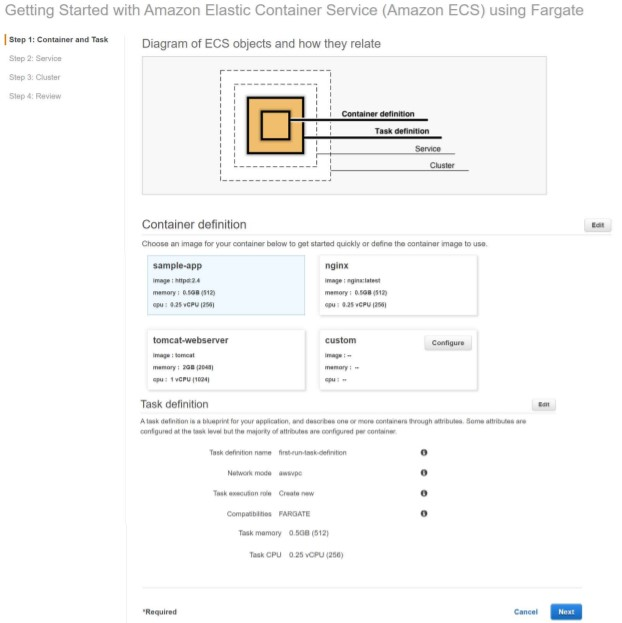
\includegraphics[width=15cm]{./images/11} 
	\end{center}
	
	
		
	\newpage
\textbf{1.11. Clic en Next.
}

    \begin{center}
		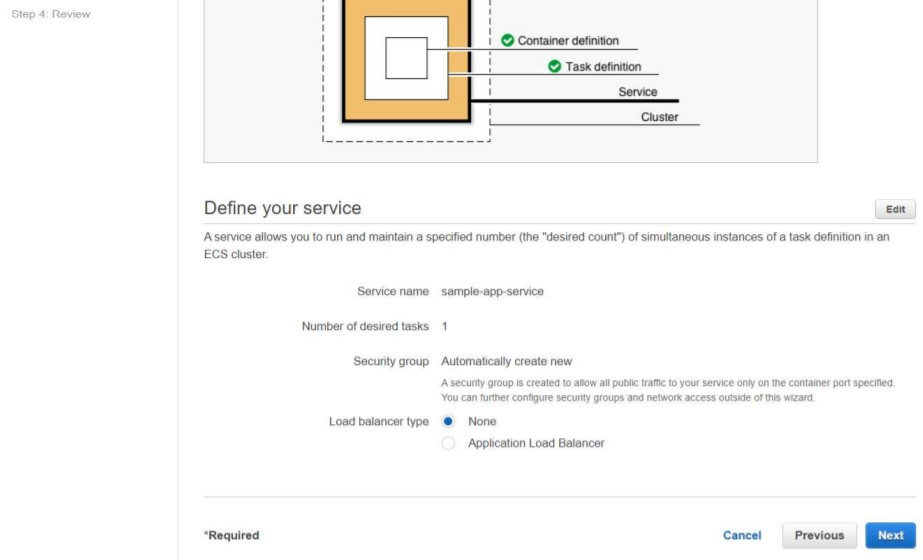
\includegraphics[width=15cm]{./images/12} 
	\end{center}
	
	
	\textbf{1.12. Clic en Next.
}

    \begin{center}
		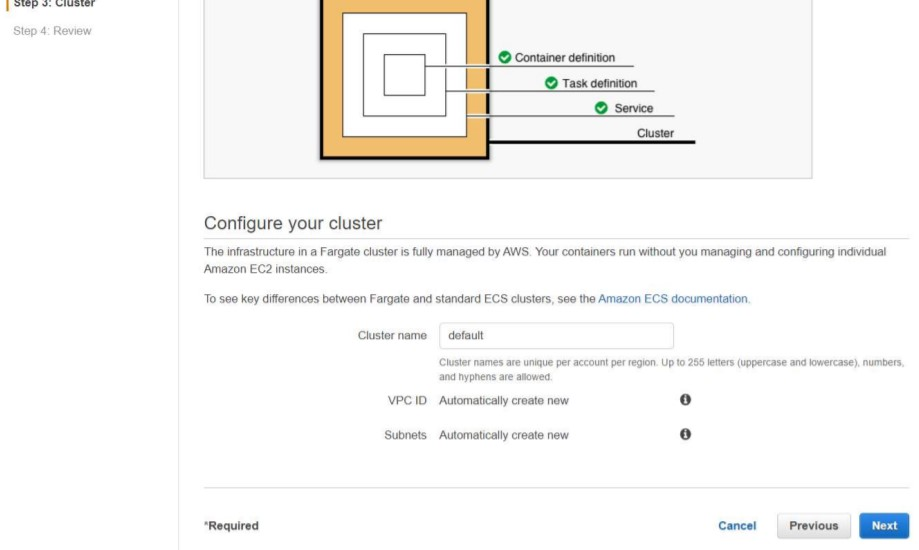
\includegraphics[width=15cm]{./images/13} 
	\end{center}
	
	\textbf{1.13.  Clic en Create
}

    \begin{center}
		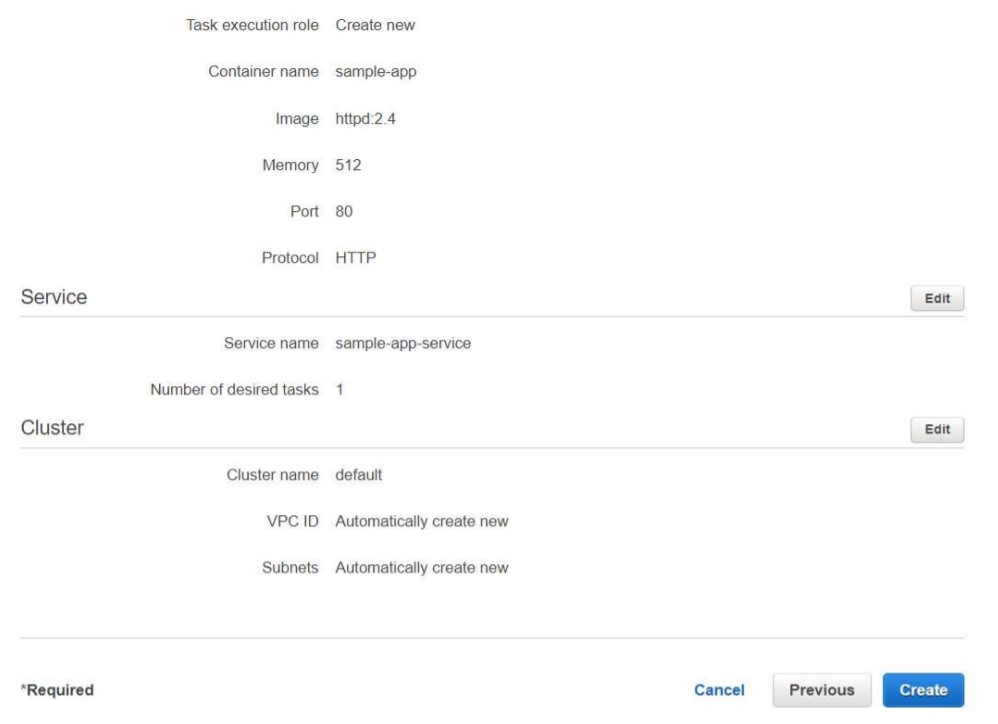
\includegraphics[width=15cm]{./images/14} 
	\end{center}
	
	\textbf{1.14. Creamos una definición de tarea.
}

    \begin{center}
		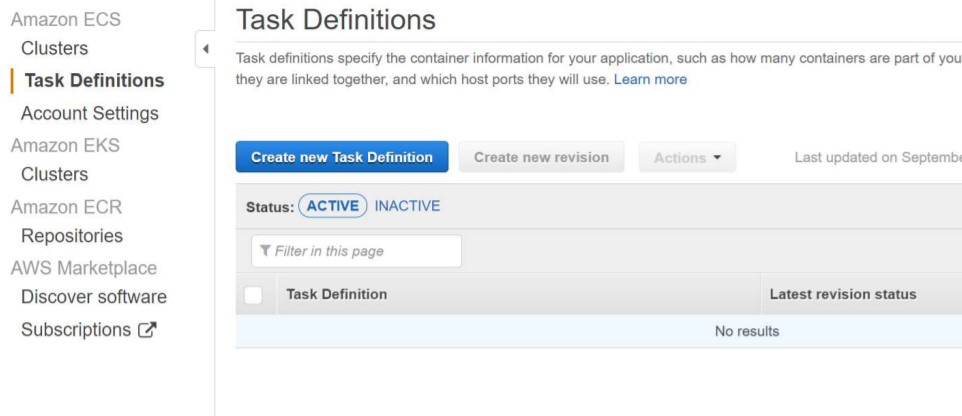
\includegraphics[width=15cm]{./images/15} 
	\end{center}
	
	\textbf{1.15.  Clic en Fargate
}

    \begin{center}
		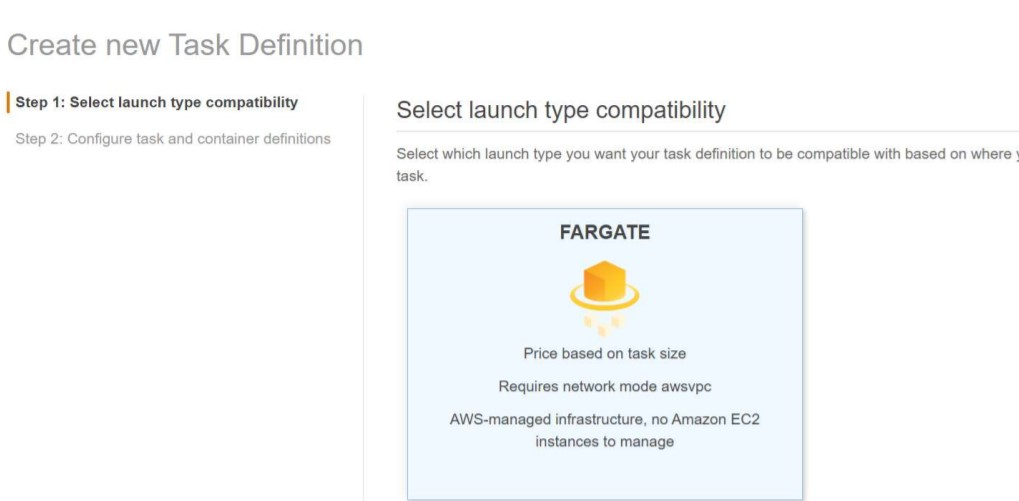
\includegraphics[width=15cm]{./images/16} 
	\end{center}
	
	\textbf{1.16.  Elegir un nombre para el task definition.
}

    \begin{center}
		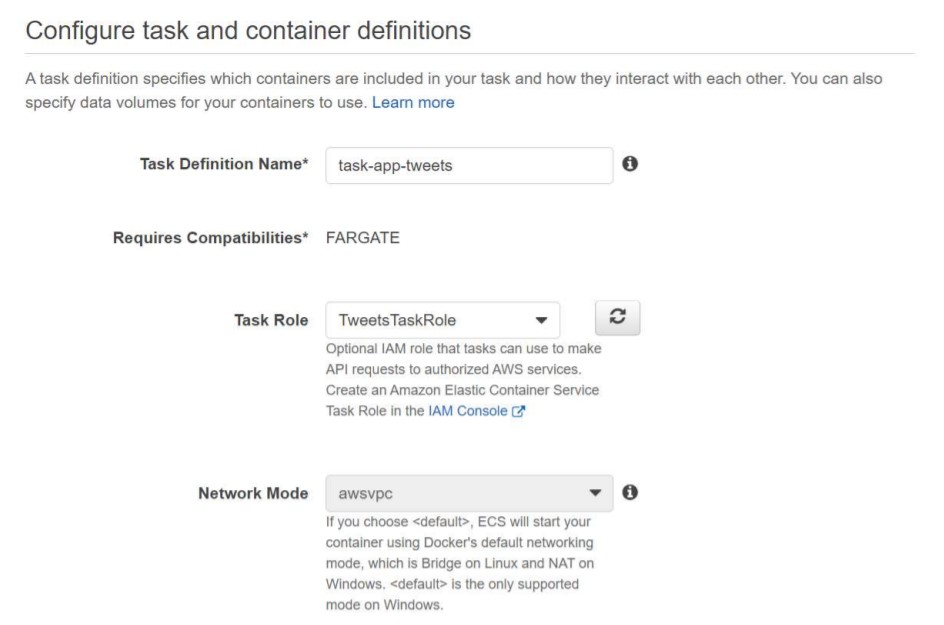
\includegraphics[width=15cm]{./images/17} 
	\end{center}
	   \begin{center}
		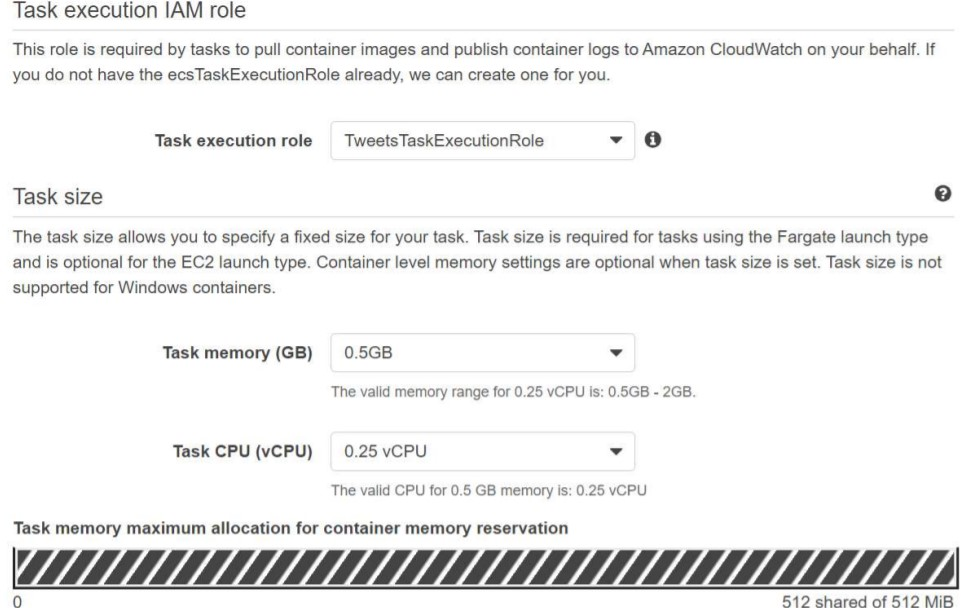
\includegraphics[width=15cm]{./images/18} 
	\end{center}
	
	
		\textbf{1.17.  Agregar el contenedor a desplegar en Fargate.
}

    \begin{center}
		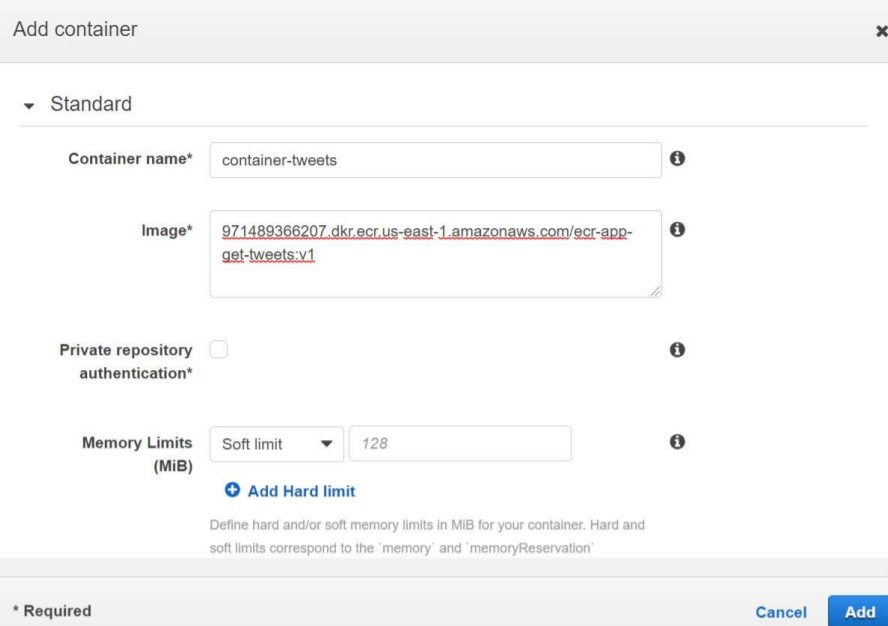
\includegraphics[width=15cm]{./images/19} 
	\end{center}
	
	
	
		\textbf{1.18. Clic en crear.
}

    \begin{center}
		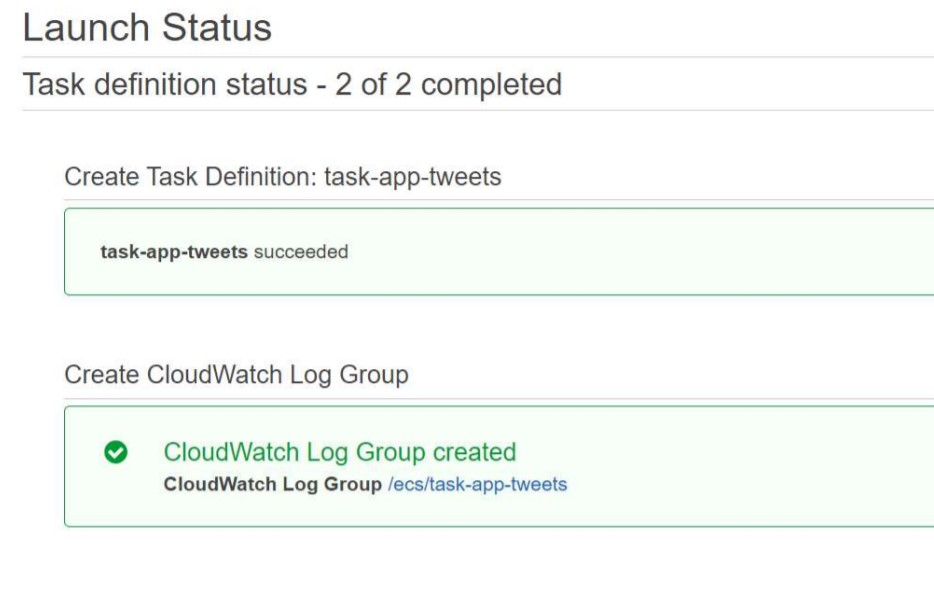
\includegraphics[width=15cm]{./images/20} 
	\end{center}
	
	
		\textbf{1.19.  Ejecutar el task definition, clic en Action -> Run task.
}

    \begin{center}
		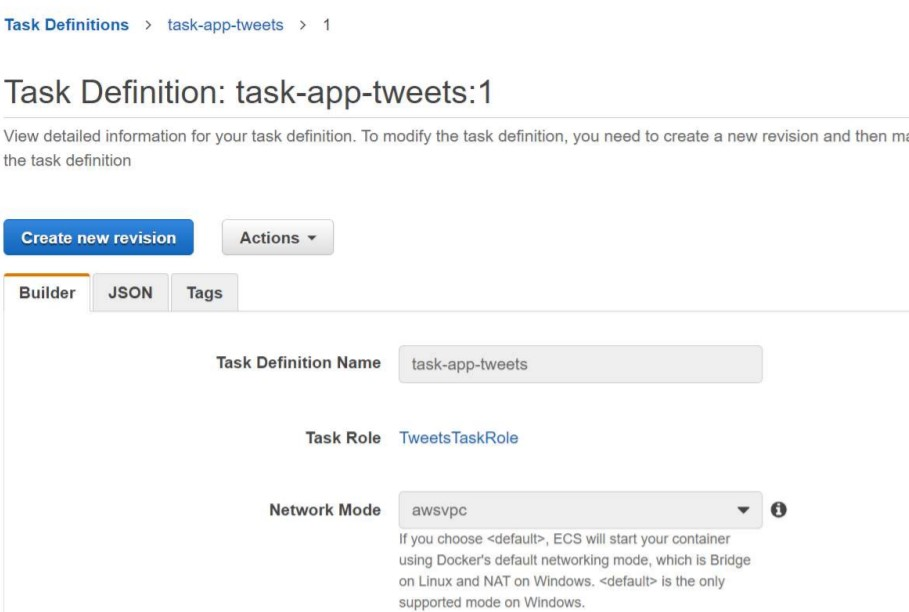
\includegraphics[width=15cm]{./images/21} 
	\end{center}
	
	
		\textbf{1.20.  Elegir el lanzamiento por Fargate.
}

    \begin{center}
		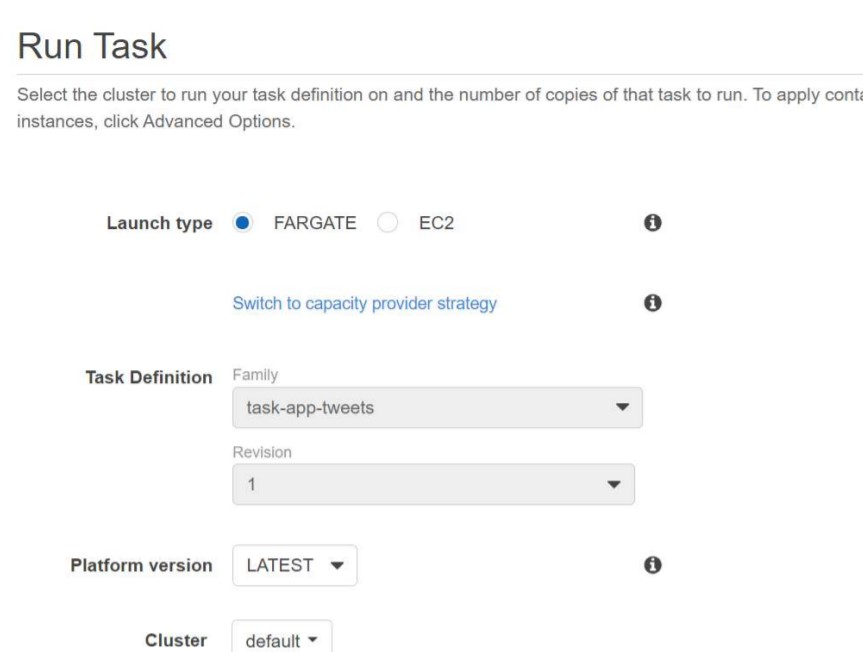
\includegraphics[width=15cm]{./images/22} 
	\end{center}
	
    \begin{center}
		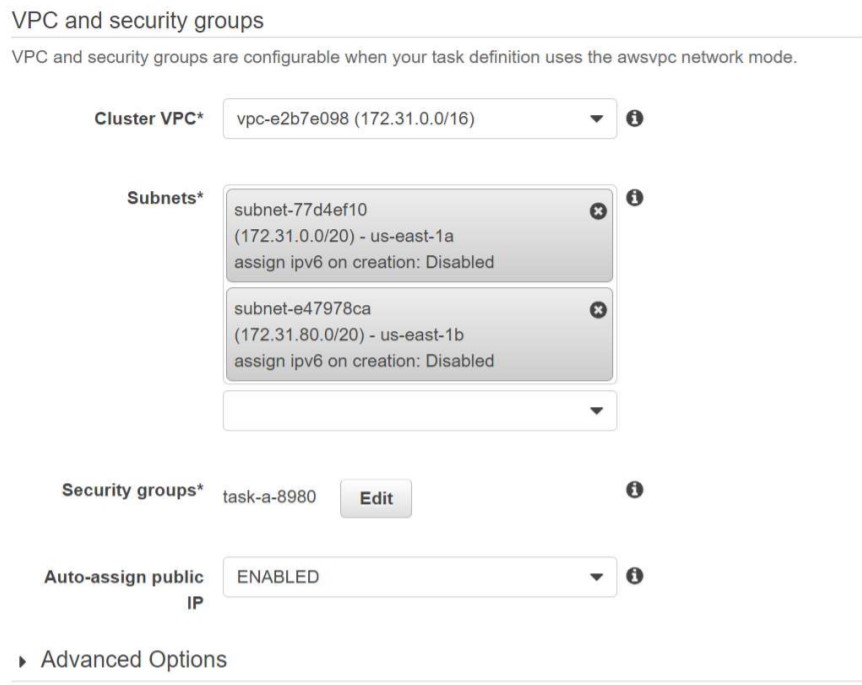
\includegraphics[width=15cm]{./images/23} 
	\end{center}
	
	
		\textbf{1.21. El task definition ya se está ejecutando.}

    \begin{center}
		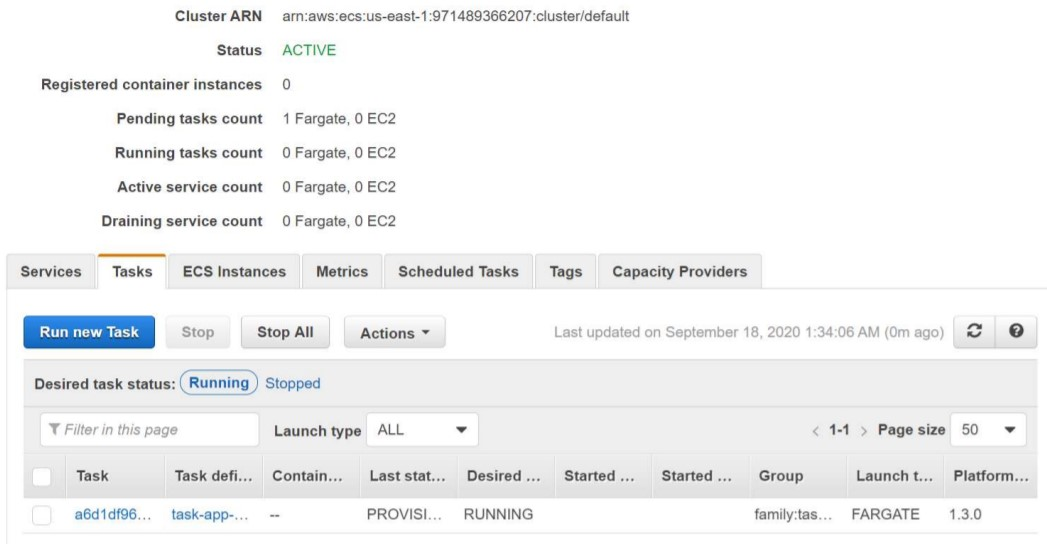
\includegraphics[width=15cm]{./images/24} 
	\end{center}
	
	
		\textbf{1.22.  Ahora acceder al servicio de ElasticSearch.
Clic en Acciones -> Modificar política de acceso
}

    \begin{center}
		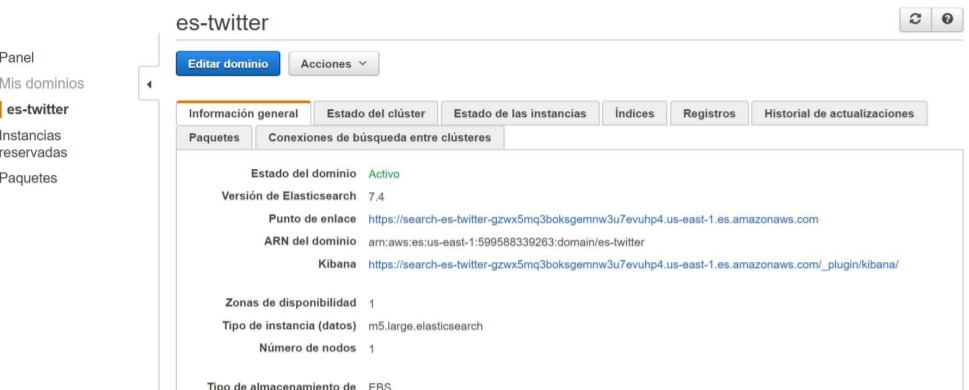
\includegraphics[width=15cm]{./images/25} 
	\end{center}
	
	
	
\end{document}